\par Les modèles décrits dans cette section appartiennent à la première classe (REF CLASSES), et ont pour objectif de prédire les longueurs de liaisons entre des atomes de carbone. Ils sont tous des réseaux de neurones artificiels entraînés avec les paramètres suivants. Le rôle de chaque paramètre est décrit en REF NN PARAMS.

\begin{figure}[!h]
	\centering
	\begin{tabular}{|l|l|}
		\hline
		\textbf{Paramètre} & \textbf{Valeur} \\ \hline
		Taille de lot (\emph{batch size}) & 5000 \\ \hline
		Epsilon (Adam) & 0.001 \\ \hline
		Initialisation des poids (\emph{stddev\_init}) & 0.001 \\ \hline
		Fonction d'activation couches cachées & elu \\ \hline
		Fonction d'activation couche de sortie & linéaire \\ \hline
		Abandon (\emph{dropout}) & 0.98 \\ \hline
		Dégradation des coefficients (\emph{weight decay}) & 0.001 \\ \hline
	\end{tabular}

	\caption{Paramètres d'entraînement des modèles \emph{DIST\_REL\_C}}
\end{figure}

\par Les tailles des jeux de données utilisés par les modèles sont donnés dans le tableau suivant. Notons que tous les modèles apprennent sur les mêmes molécules et sont testés sur les mêmes molécules, même si la préparation des données diffère.

\begin{figure}[!h]
	\centering
	\begin{tabular}{|l|l|}
		\hline
		\textbf{Jeu} & \textbf{Taille} \\ \hline
		Entraînement & 2770924 \\ \hline
		Test & 554434 \\ \hline
	\end{tabular}
	\caption{Taille des jeux de données pour les modèles \emph{DIST\_REL\_C}}
\end{figure}


\subsection{Modèle naïf}

\subsubsection{Préparation des données et paramètres}
Le premier modèle entraîné utilise la représentation locale des liaisons covalentes (REF REPR LOCALE + REF REPR DONNEES) simple, c'est à dire que l'on ne restreint pas la représentation aux atomes au voisinage le plus proche, et que l'on n'applique pas de fonction inversant l'ordre des distances. Les paramètres spécifiques d'entraînement et de préparation des données sont donnés dans le tableau suivant.


\begin{figure}[!h]
	\centering
	\begin{tabular}{|l|l|}
		\hline
		\textbf{Paramètre} & \textbf{Valeur} \\ \hline
		Taux d'apprentissage (\emph{learning rate}) & 0.01 \\ \hline
		Taille de l'entrée & 870 \\ \hline
		Taille de la dernière couche cachée & 870 \\ \hline
		Profondeur & 3 \\ \hline
		Fonction appliquée aux distances & identité \\ \hline
		Restriction du voisinage ($\epsilon$) & $\infty$ \\ \hline
	\end{tabular}

	\caption{Paramètres d'entraînement et de préparation des données spécifiques au modèle \emph{DIST\_REL\_C\_01}}
\end{figure}

\subsubsection{Analyse statistique des erreurs}
\par Dans la figure suivante, nous présentons les valeurs d'un certain nombre de métriques statistiques permettant d'évaluer les erreurs du modèle. On remarque que les prédictions du modèle sont assez bonnes, la médiane des erreurs étant de l'ordre du demi picomètre. L'erreur moyenne est toutefois au dessus de la barre du picomètre et l'erreur maximale est élevée.

\begin{figure}[!h]
	\centering
	\begin{tabular}{|l|r|}
		\hline
		\textbf{Métrique} & \textbf{Valeur} \\ \hline
		Moyenne & 1,3301 \\ \hline
		Médiane & 0,6881 \\ \hline
		Écart-type & 1,9810 \\ \hline
		Minimum & 0,0000 \\ \hline
		Maximum & 28,7268\\ \hline
		Erreur relative moyenne & 0,9126\% \\ \hline
	\end{tabular}
	
	\caption{Analyse statistique des erreurs du modèle \emph{DIST\_REL\_C\_01} (en pm)}
\end{figure}

\subsubsection{Représentation graphique des résultats}
\par La représentation graphique de la distribution des erreurs montre qu'un grand nombre d'erreurs ont des valeurs au delà du seuil du picomètre de précision nécessaire.

\begin{figure}[!h]
	\centering
	
	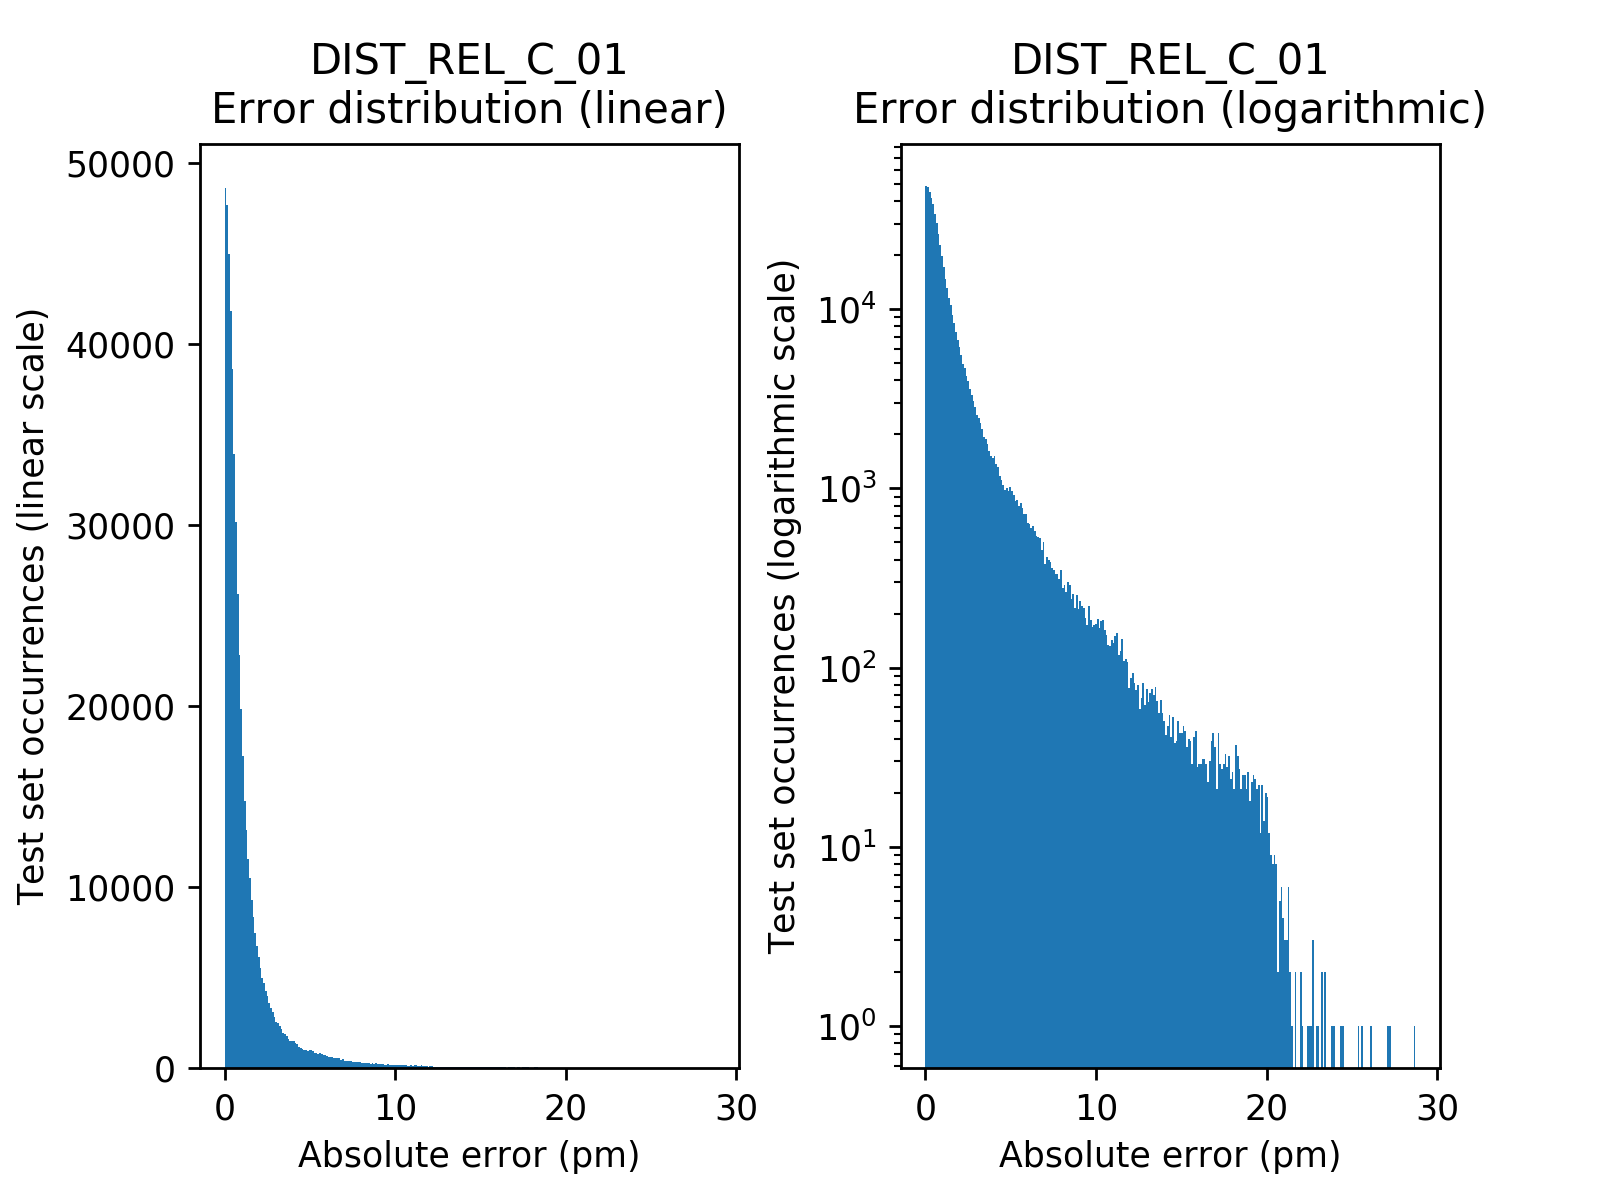
\includegraphics[scale=0.7]{../figures/DIST_REL_C_01/DIST_REL_C_01_distrib_rmse_val.png}	
	
	\caption{Distribution des erreurs du modèle \emph{DIST\_REL\_C\_01}}
\end{figure}

\par La représentation de l'erreur relative à la distance devant être prédite, exprimée en fonction des distances cibles montre que les plus grosses erreurs sont effectuées lors de la prédiction des longueurs de liaisons les moins représentées dans les données, mais que les longueurs de liaisons les plus représentées sont en revanche très bien prédites. L'histogramme de la représentation des liaisons situé dans la partie inférieure permet de s'en rendre compte.

\begin{figure}[!h]
	\centering
	
	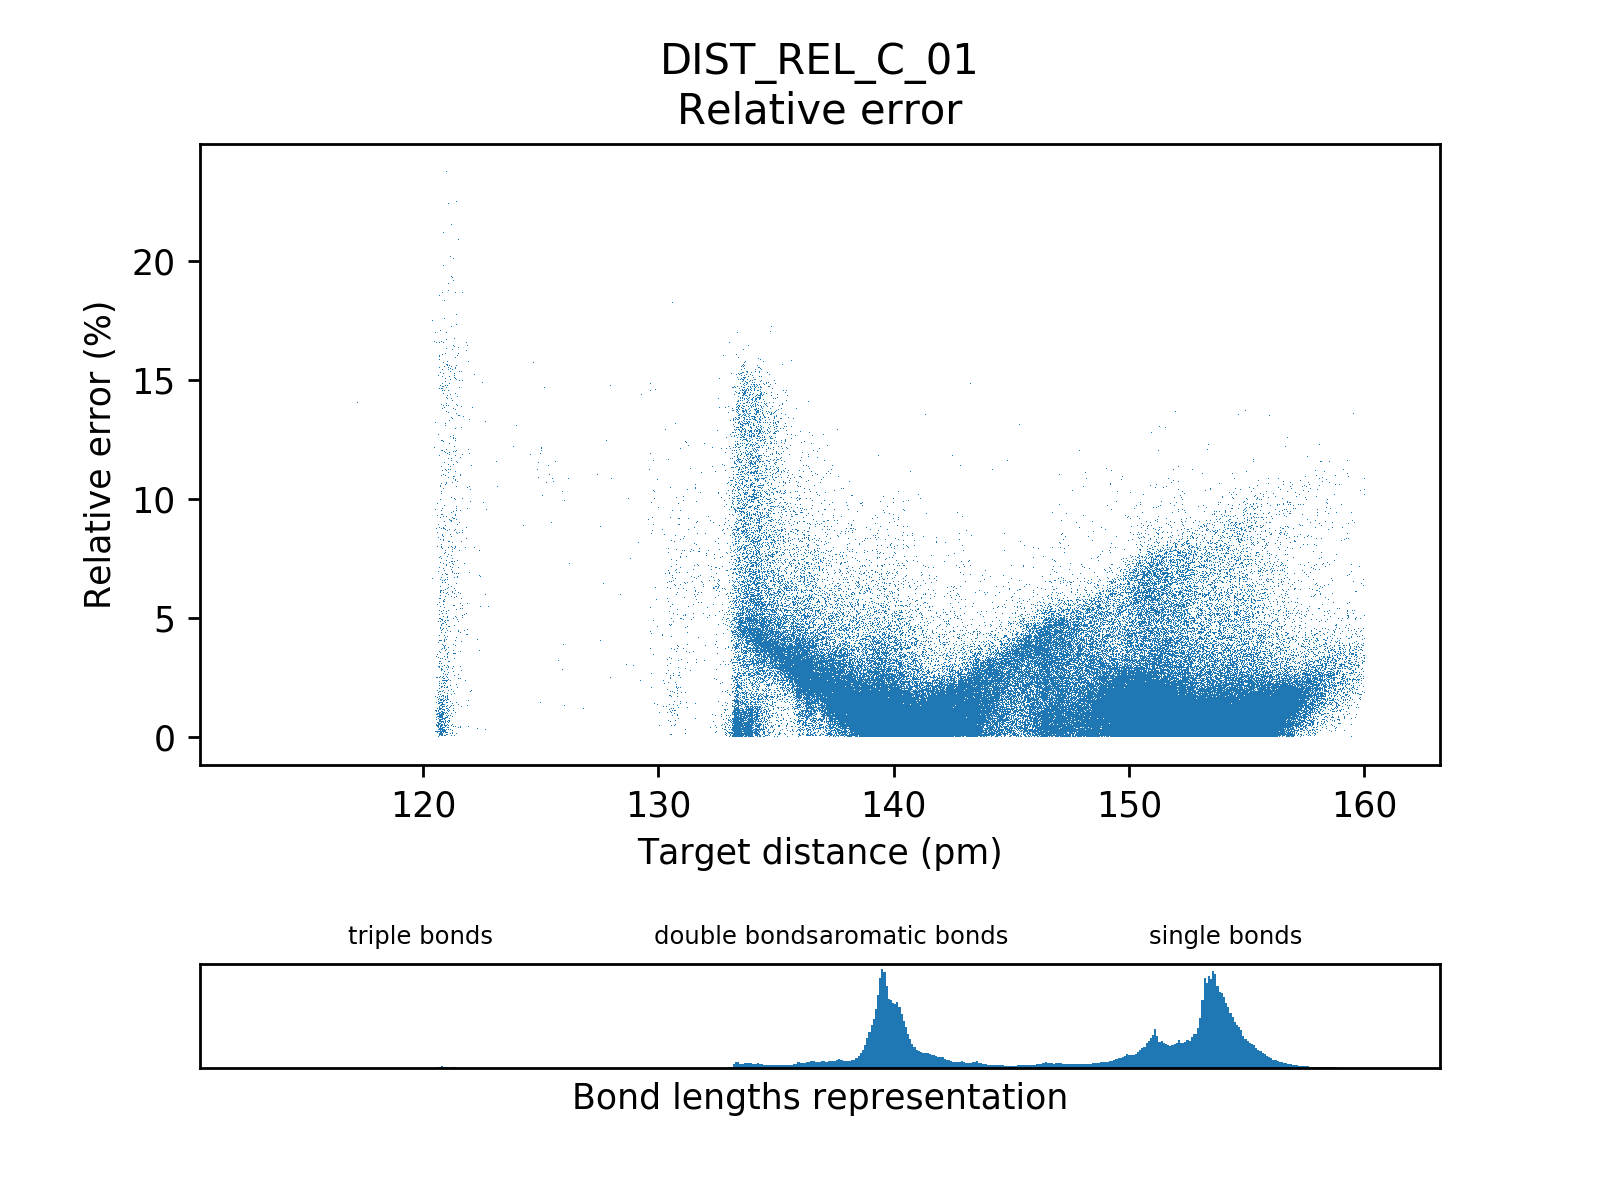
\includegraphics[scale=0.7]{../figures/DIST_REL_C_01/DIST_REL_C_01_distrib_rmse_dist.png}	
	
	\caption{Erreur en fonction des cibles pour le modèle \emph{DIST\_REL\_C\_01}}
\end{figure}

\par Enfin, la représentation des prédictions en fonction des distances cibles permet de préciser quels types d'erreurs sont commises en fonction des différentes classes de liaisons à prédire. Les liaisons doubles et triples sont très largement surestimées, même si une partie non négligeable de ces liaisons est correctement prédite. La grande majorité des liaisons simples et aromatiques sont très bien prédites, même si une partie des liaisons aromatiques est légèrement sur-estimée et une partie des liaisons simples est légèrement sous-estimée.\\

\begin{figure}[!h]
	\centering
	
	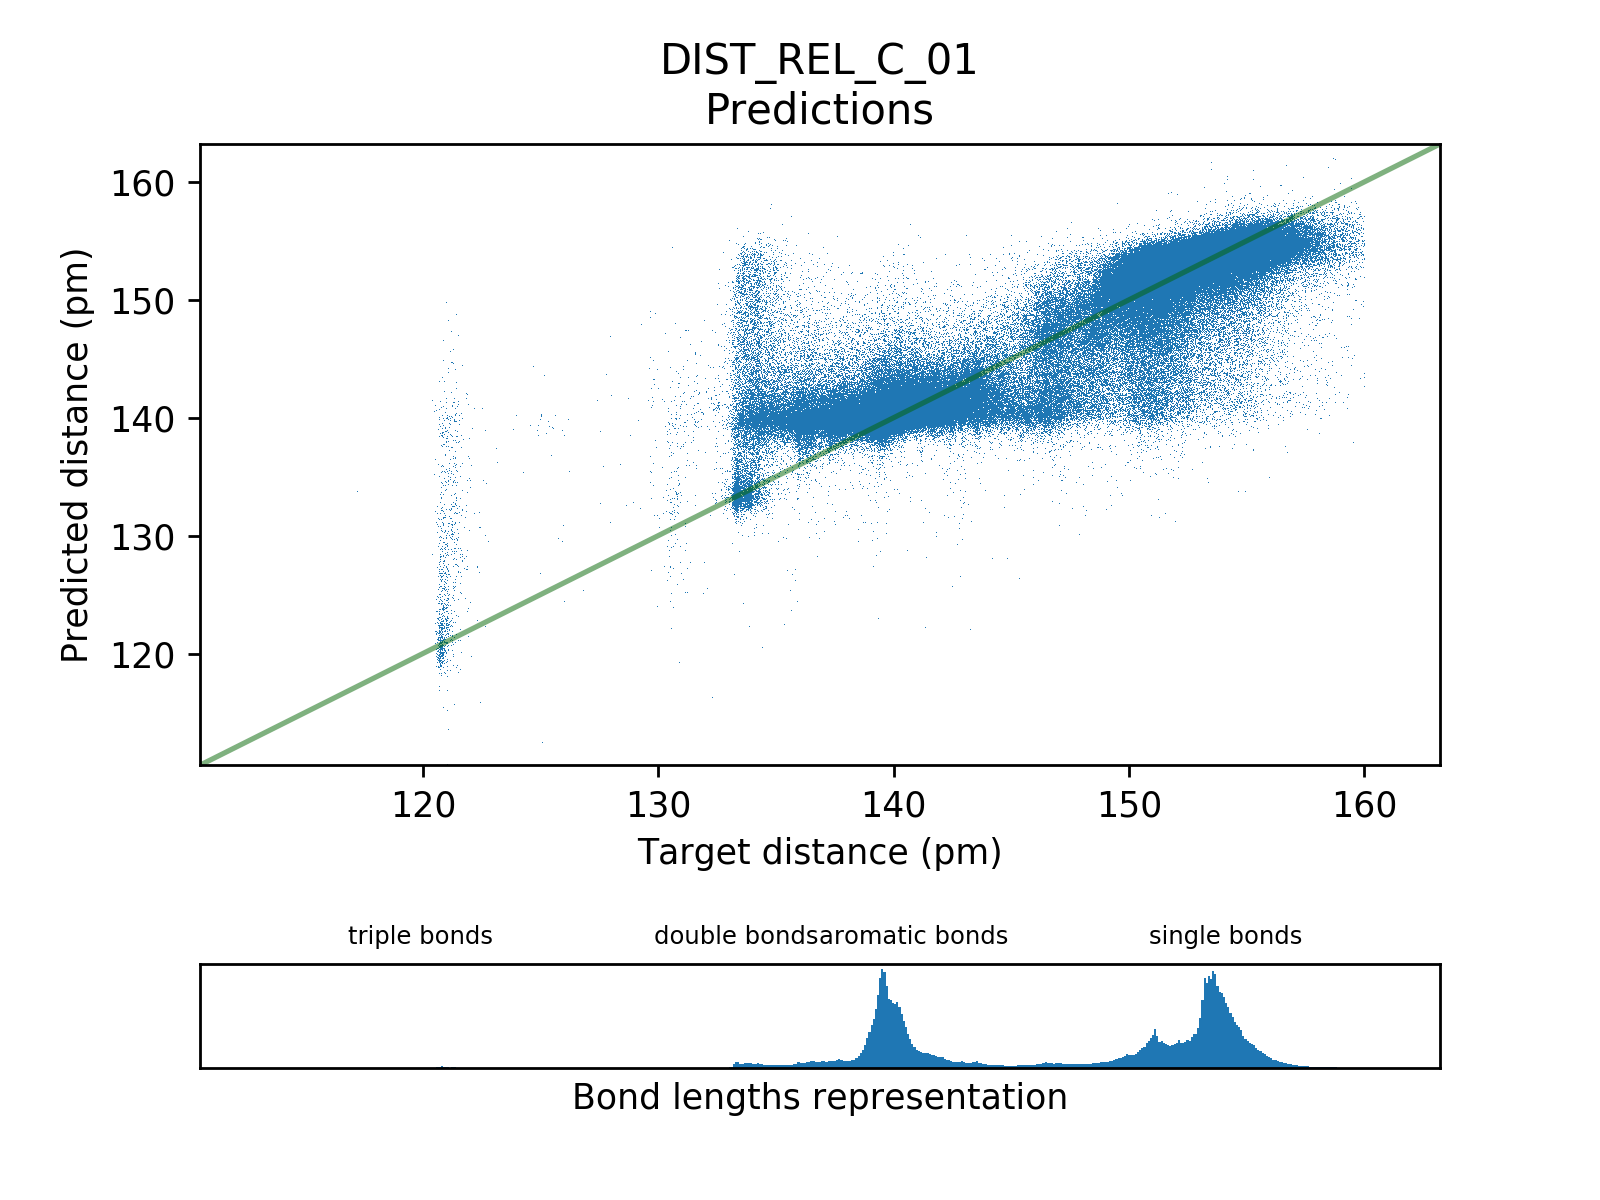
\includegraphics[scale=0.7]{../figures/DIST_REL_C_01/DIST_REL_C_01_preds_targets.png}	
	
	\caption{Prédictions en fonction des cibles pour le modèle \emph{DIST\_REL\_C\_01}}
	
\end{figure}

\subsection{Restriction au voisinage le plus proche}

\subsubsection{Préparation des données et paramètres}
À la différence du modèle naïf qui a en entrée tous les atomes d'une molécule (à l'exception des deux atomes formant la liaison étudiée), nous limitons l'entrée de ce modèle aux atomes au voisinage proche de la liaison (REF RESTRICTION VOISINAGE). Cela a pour objectif de donner uniquement l'information la plus pertinente, et donc de guider le modèle vers de meilleures solutions. Les paramètres spécifiques de préparation des données et d'entraînement sont donnés dans le tableau suivant.

\begin{figure}[!h]
	\centering
	\begin{tabular}{|l|l|}
		\hline
		\textbf{Paramètre} & \textbf{Valeur} \\ \hline
		Taux d'apprentissage (\emph{learning rate}) & 0.01 \\ \hline
		Taille de l'entrée & 870 \\ \hline
		Taille de la dernière couche cachée & 870 \\ \hline
		Profondeur & 3 \\ \hline
		Fonction appliquée aux distances & identité \\ \hline
		Restriction du voisinage ($\epsilon$) & 200 pm \\ \hline
	\end{tabular}

	\caption{Paramètres d'entraînement et de préparation des données spécifiques au modèle \emph{DIST\_REL\_C\_01}}
\end{figure}

\subsubsection{Analyse statistique des erreurs}
\par Le tableau suivant présente les différentes valeurs des métriques statistiques utilisées pour évaluer les erreurs des modèles. Ses performances sont très intéressantes puisque la moyenne comme la médiane sont en dessous du picomètre. Le modèle semble toutefois toujours faire de grosses erreurs, même si l'erreur maximale a diminué de moitié.

\begin{figure}[!h]
	\centering
	\begin{tabular}{|l|r|}
		\hline
		\textbf{Métrique} & \textbf{Valeur} \\ \hline
		Moyenne & 0,5146 \\ \hline
		Médiane & 0,4225 \\ \hline
		Écart-type & 0,5022 \\ \hline
		Minimum & 0,0000 \\ \hline
		Maximum & 102,3328\\ \hline
		Erreur relative moyenne & 0,3472\% \\ \hline
	\end{tabular}
	
	\caption{Analyse statistique des erreurs du modèle \emph{DIST\_REL\_C\_02} (en pm)}
\end{figure}

\subsubsection{Représentation graphique des résultats}
\par La représentation graphique de la distribution des erreurs montre que le modèle est très intéressant, les erreurs au-delà de 10 pm étant marginales. \\

\begin{figure}[!h]
	\centering
	
	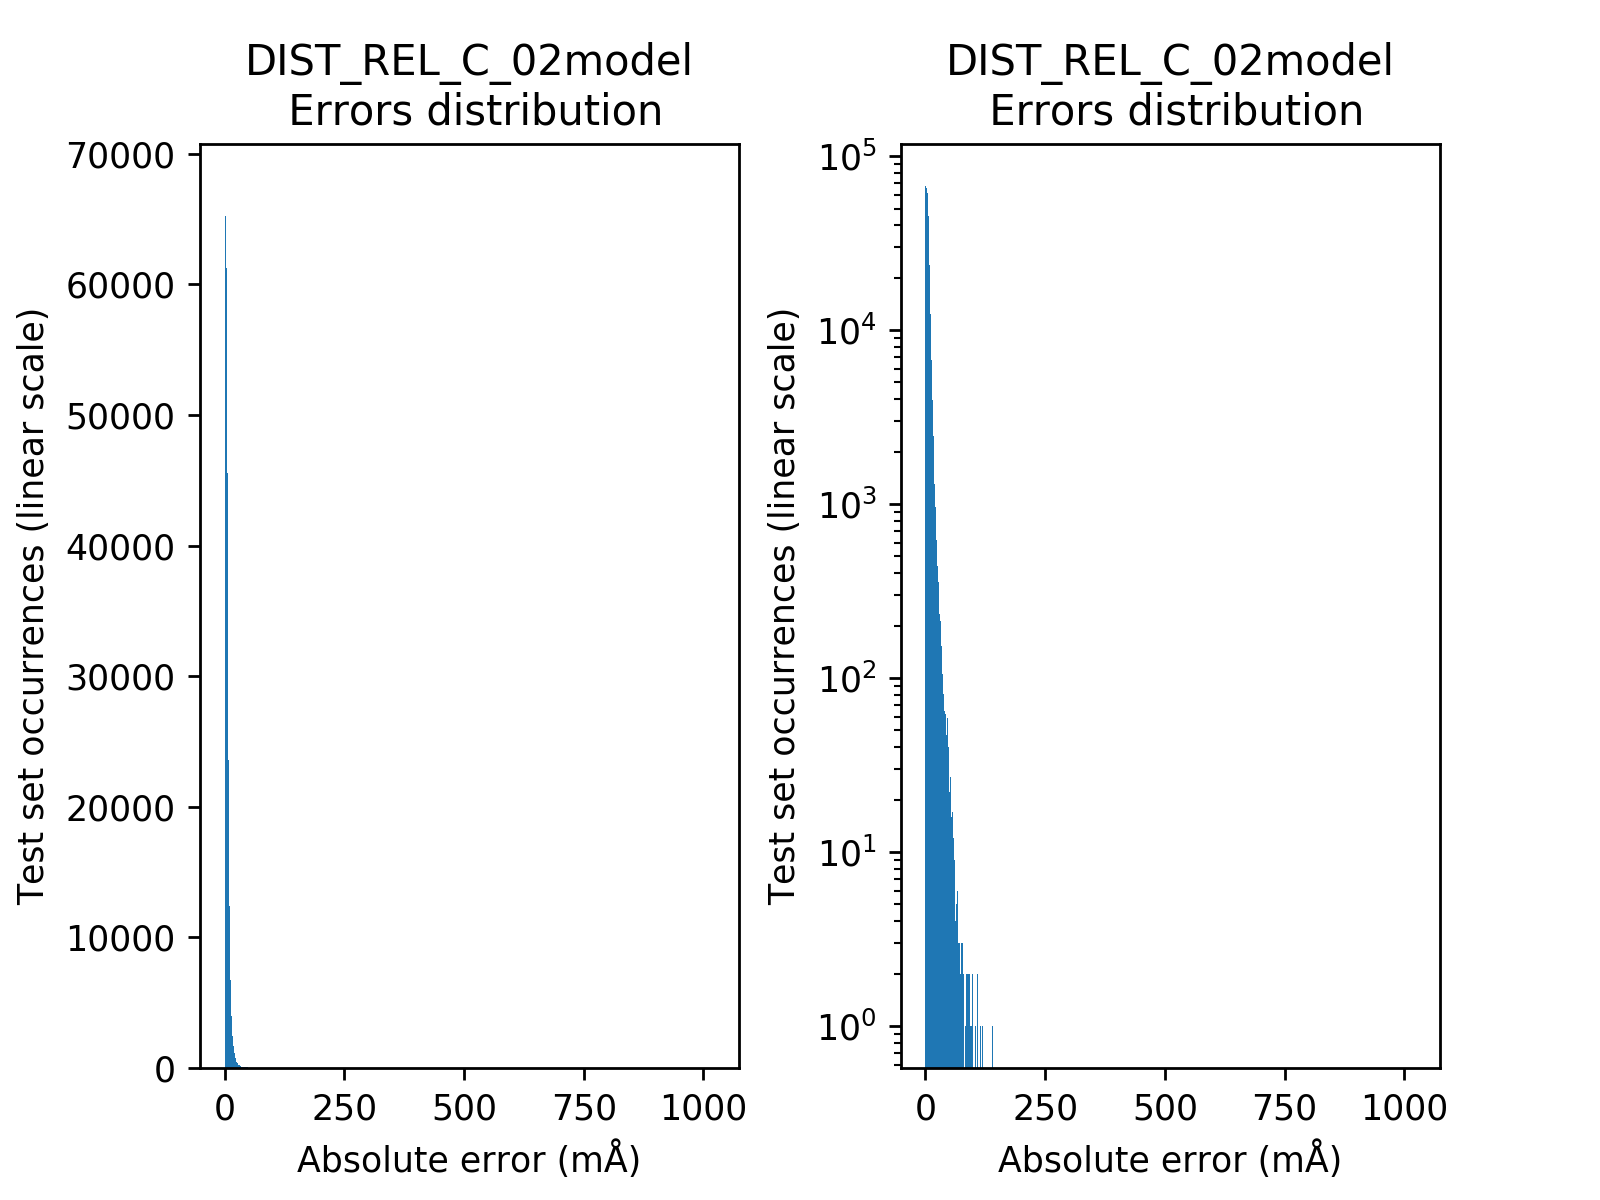
\includegraphics[scale=0.7]{../figures/DIST_REL_C_02/DIST_REL_C_02_distrib_rmse_val.png}	
	
	\caption{Distribution des erreurs du modèle \emph{DIST\_REL\_C\_02}}
\end{figure}

\par La représentation graphique de l'erreur en fonction des cibles montre également nettement l'intérêt du modèle. En effet, il ne fait plus d'erreurs importantes sur les liaisons aux tailles limites entre les liaisons aromatiques et simples. \\

\begin{figure}[!h]
	\centering
	
	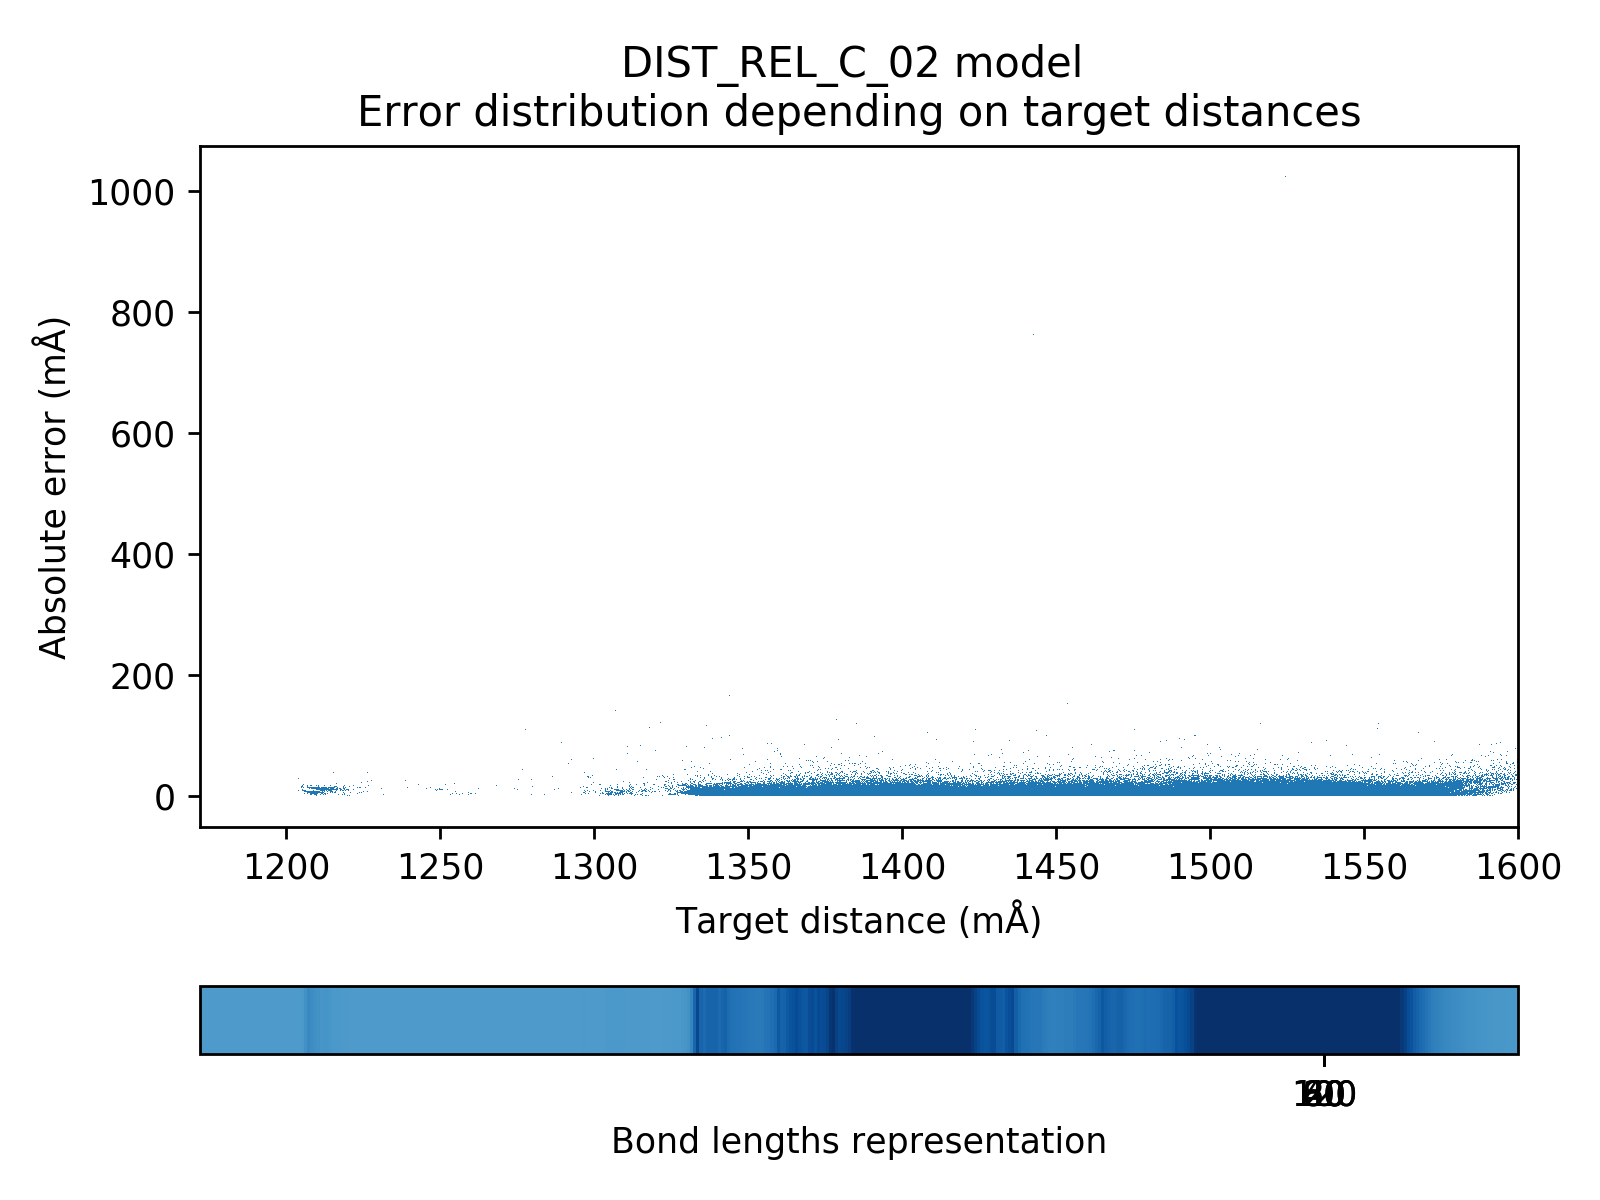
\includegraphics[scale=0.7]{../figures/DIST_REL_C_02/DIST_REL_C_02_distrib_rmse_dist.png}	
	
	\caption{Erreur en fonction des cibles pour le modèle \emph{DIST\_REL\_C\_02}}
	\end{figure}

\par Enfin, la représentation des prédictions en fonction des cibles confirme la continuité des prédictions du modèle entre les différents types de liaisons, ce qui confirme qu'il effectue des prédictions de l'ordre de la chimie quantique, et qu'il ne se contente pas de faire des prédictions basées sur des longueurs de liaisons types.
\begin{figure}[!h]
	\centering
	
	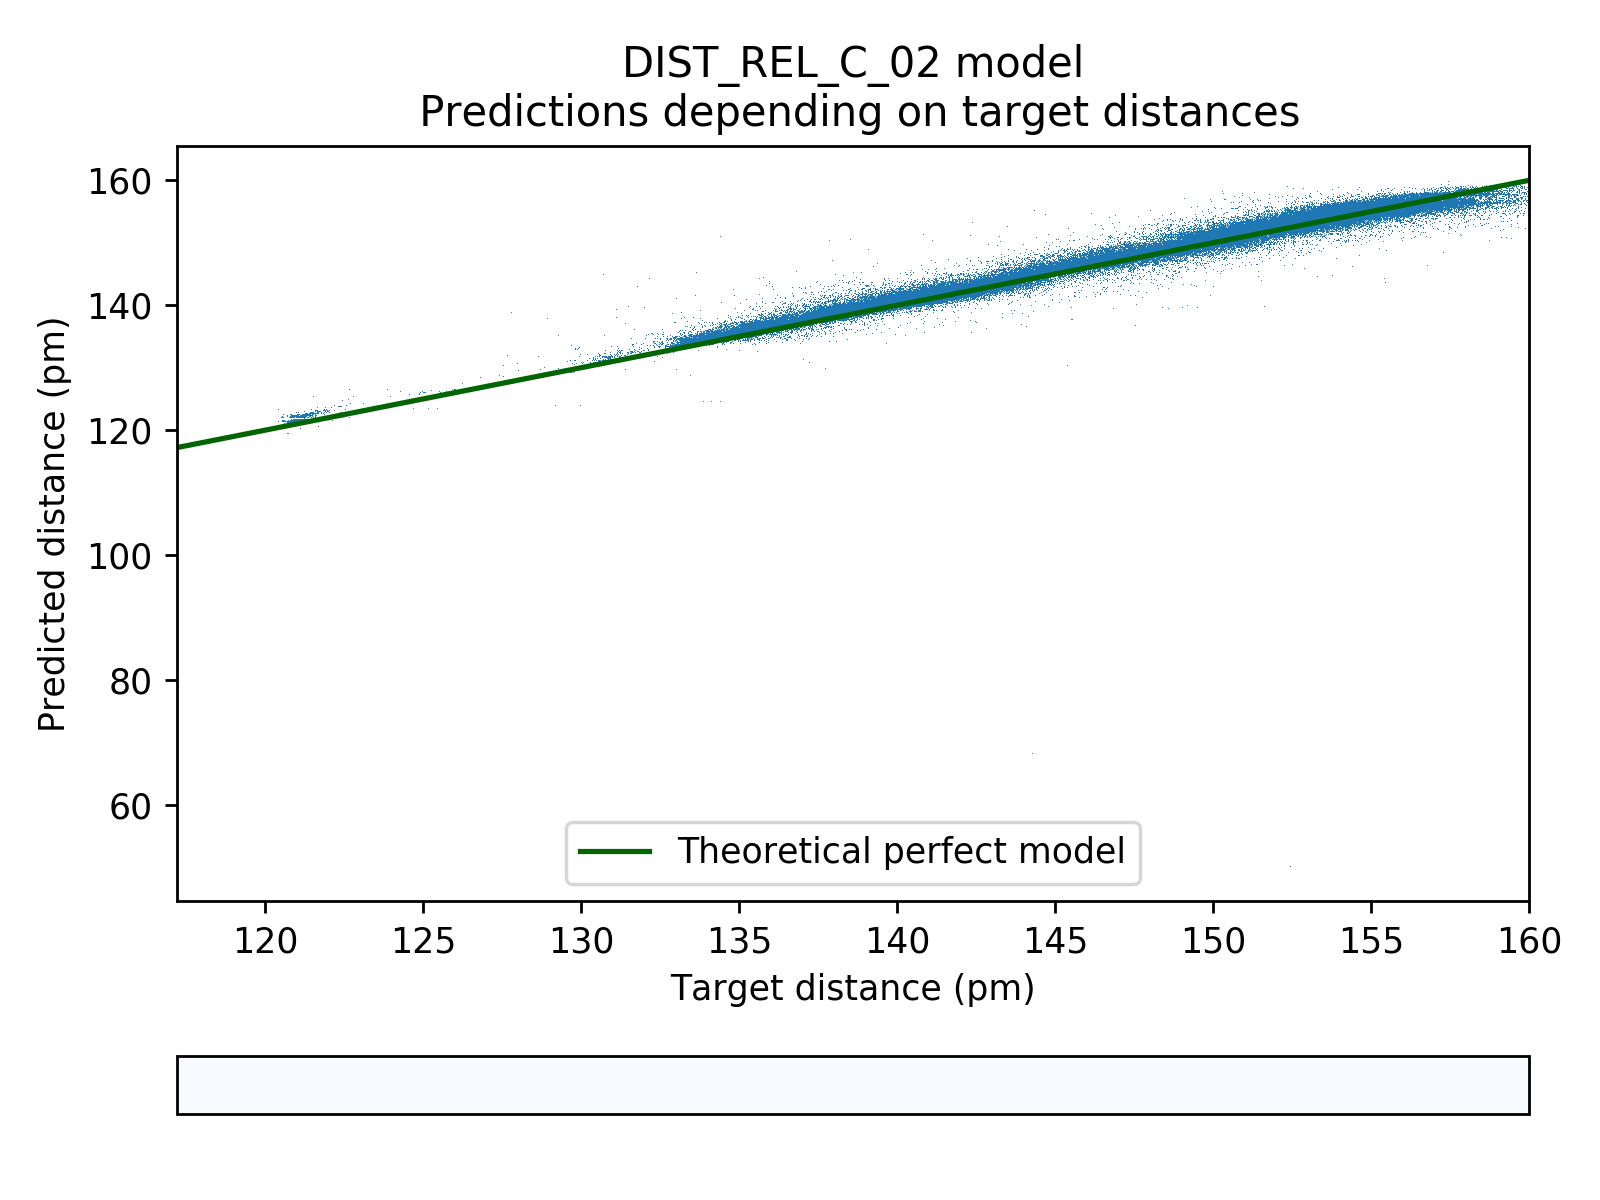
\includegraphics[scale=0.7]{../figures/DIST_REL_C_02/DIST_REL_C_02_preds_targets.png}	
	
	\caption{Prédictions en fonction des cibles pour le modèle \emph{DIST\_REL\_C\_02}}
	
\end{figure}

\subsection{Application de fonctions aux distances}

\subsubsection{Préparation des données et paramètres}
Les deux modèles décrits dans cette section sont identiques à \emph{DIST\_REL\_C\_02}, à la différence qu'une fonction inversant l'ordre des distances aux atomes de la liaison est appliquée aux données d'entrée (REF FONCT). Cette fonction a pour objectif de guider les modèles vers de meilleures solutions, l'influence des atomes sur la longueur de la liaison étant inversement proportionnelle à leur distance à la liaison. Les résultats des modèles s'en voient améliorés, mais nous montrons en REF XY FONCTIONS que les modèles s'entraînant sur plus d'exemples sont en général plus performants lorsque aucune fonction n'est appliquée aux distances.\\
Les paramètres d'entraînement spécifiques des deux modèles sont donnés dans la figure suivante.

\begin{figure}[!h]

	\centering
	\begin{tabular}{|l|l|l|}
		\hline
		\textbf{Paramètre} & \multicolumn{2}{|c|}{\textbf{Valeur}} \\ 
		 & \emph{DIST\_REL\_C\_03} & \emph{DIST\_REL\_C\_04} \\ \hline
		Taux d'apprentissage (\emph{learning rate}) & 0.01 & 0.01\\ \hline
		Taille de l'entrée & 870 & 870\\ \hline
		Taille de la dernière couche cachée & 870 & 870\\ \hline
		Profondeur & 3 & 3\\ \hline
		Fonction appliquée aux distances & inverse & inverse du carré\\ \hline
		Restriction du voisinage ($\epsilon$) & 2 pm & 2 pm\\ \hline
	\end{tabular}
	
	\caption{Paramètres d'entraînement et de préparation des données spécifiques aux modèles}
\end{figure}

\subsubsection{Analyse statistique des erreurs}

Le tableau suivant présente les valeurs des métriques statistiques permettant d'évaluer les erreurs pour les deux modèles. En comparaison au modèle \emph{DIST\_REL\_C\_02}, les deux modèles ont des erreurs maximales largement inférieures. L'utilisation de la fonction inverse fait en revanche augmenter la valeur de toutes les autres métriques. La fonction inverse du carré semble plus prometteuse, car elle fait baisser la moyenne et la médiane. L'écart-type est en revanche légèrement supérieur. Ces différences statistiques étant subtiles, elles sont à prendre avec le recul nécessaire lié au fait que l'on compare des exécutions uniques. Pour s'assurer que ces différences sont constantes, il faudrait entraîner chaque modèle une dizaine de fois et étudier les différentes valeurs de chaque métrique, ce qui représenterait quelques jours d'exécution.\\

Les représentations graphiques étant très similaires à celles du modèle \emph{DIST\_REL\_C\_02}, nous ne les affichons pas ici. Elles sont néanmoins disponibles en annexes (REF ANNEXES DIST\_REL\_C\_034).

\begin{figure}[!h]
	\centering
	\begin{tabular}{|l|r|r|}
		\hline
		\textbf{Métrique}& \textbf{\emph{DIST\_REL\_C\_03}} & \textbf{\emph{DIST\_REL\_C\_04}} \\ \hline
		Moyenne & 0,6255 & 0,4743\\ \hline
		Médiane & 0,6255 & 0,3086 \\ \hline
		Écart-type & 0,6434 & 0,5521 \\ \hline
		Minimum & 0,0000 & 0,0000\\ \hline
		Maximum & 15,479431 & 17,5180\\ \hline
		Erreur relative moyenne & 0,4226\% & 0,3198\%\\ \hline
	\end{tabular}
	
	\caption{Analyse statistique des erreurs des modèles (en pm)}
\end{figure}

\subsection{Réduction de la largeur du réseau et des entrées}
\par Les modèles précédents sont très performants, mais ont l'inconvénient de nécessiter un temps d'entraînement élevé. C'est d'autant plus vrai pour les modèles de la seconde classe équivalents (REF INTRO CLASSES ET REF GENERALISATION). Pour tenter d'accélérer les processus d'entraînement, nous modifions la topologie des réseaux de neurones et nous réduisons la taille des entrées.
\par Dans les modèles précédents, l'entrée est composée de 58 blocs représentant chacun un atome au voisinage de la liaison (REF REPR DONNEES INTRO). Or depuis le modèle \emph{DIST\_REL\_C\_02}, les entrées ne sont plus composées que des atomes au voisinage le plus proche, tous les blocs ne sont donc plus nécessaires. Une recherche rapide par dichotomie du nombre de blocs tel que tous les exemples des jeux de données ont un nombre d'atomes au voisinage proche qui lui est inférieur ou égal donne une valeur de 15. L'entrée du modèle a alors une nouvelle taille de 15 blocs par 15 attributs, soit 225 attributs contre 870 auparavant.
\par La topologie des modèles précédents est simple : ils sont composés de trois couches cachées de 870 neurones artificiels. Le modèle que l'on entraîne ici est composé de trois couches cachées de tailles décroissantes. La taille des couches de l'entrée à la dernière couche décroît linéairement de 225 à 15 neurones. La valeur de la taille de cette dernière couche est choisie pour correspondre au nombre maximum d'atomes donnés en entrée, dans l'idée que les modèles pourront extraire couche par couche l'influence de chaque atome. La comparaison entre les deux topologies est donnée dans le tableau suivant.

\begin{figure}[!h]
	\centering
	\begin{tabular}{|c|r|r|}
		\hline
		& \textbf{\emph{DIST\_REL\_C\_X, X<5}} & \textbf{\emph{DIST\_REL\_C\_05}}\\ \hline
		\textbf{Taille couche entrée} & 870 & 225 \\ \hline
		\textbf{Taille première couche cachée} & 870 & 120\\ \hline
		\textbf{Taille seconde couche cachée} & 870 & 67\\ \hline
		\textbf{Taille troisième couche cachée} & 870 & 15\\ \hline
		\textbf{Taille couche sortie} & 1 & 1\\ \hline
		\textbf{Nombre de neurones artificiels} & 901 & 428\\ \hline
		\textbf{Nombre de connexions} & 152100 & 36060 \\ \hline
	\end{tabular}
	
	\caption{Comparaison de la topologie du modèle \emph{DIST\_REL\_C\_05} avec celle des modèles précédents}
\end{figure}

\par En dehors de la topologie, les paramètres d'entraînement sont identiques à ceux de \emph{DIST\_REL\_C\_02} (REF MODELE RESTRICTION).

\subsection{Recherche par quadrillage des paramètres du modèle naïf}

\par Afin d'en optimiser les performances, nous effectuons une recherche par quadrillage des paramètres du modèle \emph{DIST\_REL\_C\_01} (REF MODELE NAIF). L'entraînement de chaque modèle prenant plusieurs heures, relativement peu de paramètres différents sont testés. Les paramètres qui varient sont limités à la profondeur du réseau de neurones et au taux d'apprentissage. Chaque entraînement est effectué deux fois dans le cadre d'une validation croisée des résultats. Une validation croisée à deux entraînements ne permet pas de s'assurer de la constance des résultats, mais limite le nombre d'entraînements nécessaires et augmente donc le nombre d'ensembles de paramètres différents pouvant être testés. La performance relative des différents paramètres est évaluée à l'aide de la sortie de tensorboard (REF Tensorboard).\\

\par La recherche par quadrillage est en réalité constituée de trois sous-recherches. La grille de la première recherche est choisie arbitrairement, tandis que les grilles des autres recherches dépendent des meilleurs paramètres des recherches précédentes.

\begin{figure}[!h]
	\centering
	
	\begin{tabular}{|l|l|}
		\hline
		\textbf{Paramètres} & \textbf{Valeurs} \\ \hline 
		Taux d'apprentissage (\emph{learning rate}) & 0.01, 0.02 \\ \hline
		Profondeur & 1, 2, 3 \\ \hline
	\end{tabular}		
	
	\caption{Première grille de recherche par quadrillage pour le modèle \emph{DIST\_REL\_C\_01}}
\end{figure}

\par La sortie de tensorboard associée à la première recherche est donnée dans la figure suivante. Elle représente l'erreur moyenne de tous les modèles sur les données de validation au fil de l'entraînement. Les données d'entraînement et de validation forment deux ensembles disjoints. Pour donner un ordre de grandeur des résultats, la différence entre les performances des deux premiers modèles est de l'ordre de 0.3 pm, et la différence entre le meilleur et le pire modèle est de l'ordre de 4 pm. Les meilleurs résultats étant obtenus avec le taux d'apprentissage le plus faible et le réseau le plus profond, on définit une nouvelle grille à partir de cette nouvelle connaissance. À l'issue de la seconde recherche, on utilise la même méthode pour définir une troisième grille de recherche.
\par Notons les résultats des modèles sur les jeux de test sont meilleurs que pendant l'entraînement, à cause de de la désactivation de certains neurones à chaque époque d'entraînement (REF DROPOUT).

\vspace{0.5cm}

\begin{figure}[!h]
	\centering
	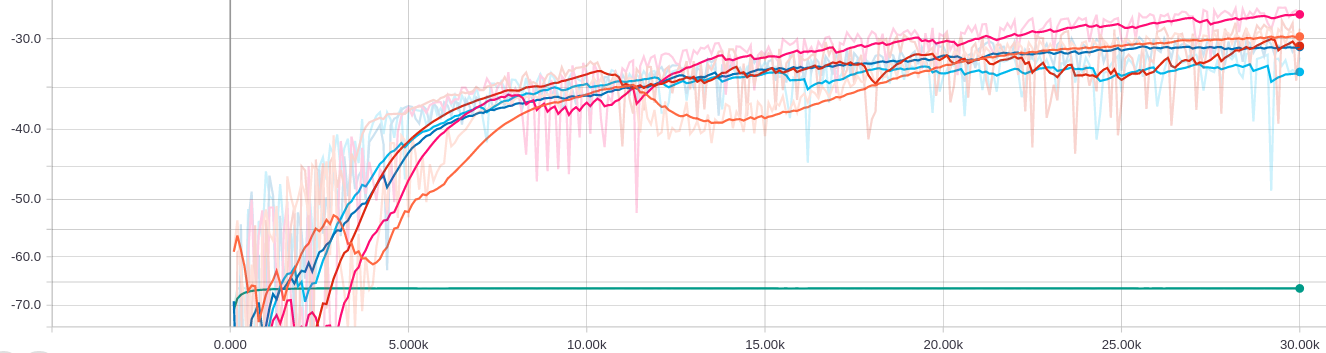
\includegraphics[scale=0.35]{images/tboard.png}
	\caption{Sortie de tensorboard pour la première recherche par quadrillage du modèle \emph{DIST\_REL\_C\_01}}
\end{figure}

\begin{figure}[!h]
	\centering
	
	\begin{tabular}{|l|l|}
		\hline
		\textbf{Paramètres} & \textbf{Valeurs} \\ \hline 
		Taux d'apprentissage (\emph{learning rate}) & 0.01\\ \hline
		Profondeur & 4, 5 \\ \hline
	\end{tabular}	
	
	\vspace{0.5cm}	
	
	\begin{tabular}{|l|l|}
		\hline
		\textbf{Paramètres} & \textbf{Valeurs} \\ \hline 
		Taux d'apprentissage (\emph{learning rate})& 0.005, 0.001\\ \hline
		Profondeur & 3 \\ \hline
	\end{tabular}
	
	\vspace{0.5cm}	

	\begin{tabular}{|l|l|}
		\hline
		\textbf{Paramètres} & \textbf{Valeurs} \\ \hline 
		Taux d'apprentissage (\emph{learning rate})& 0.005, 0.001, 0.008\\ \hline
		Profondeur & 4, 5, 6 \\ \hline
	\end{tabular}		
	\caption{Seconde grille de recherche par quadrillage pour le modèle \emph{DIST\_REL\_C\_01}}
\end{figure}
              
\begin{figure}[!h]
	\centering
	\begin{tabular}{|l|l|}
		\hline
		\textbf{Paramètres} & \textbf{Valeurs} \\ \hline 
		Taux d'apprentissage (\emph{learning rate}) & 0.001, 0.0005\\ \hline
		Profondeur & 7, 8, 9\\ \hline
	\end{tabular}	
	
	\caption{Troisième grille de recherche par quadrillage pour le modèle \emph{DIST\_REL\_C\_01}}
\end{figure}

\par La dernière recherche par quadrillage montre que les meilleures performances sont obtenues par le modèle ayant un taux d'apprentissage de 0.001 et une profondeur de 9. Pour donner un ordre de grandeur, la différence entre les performances du meilleur modèle de la première recherche par quadrillage et de la dernière est de 0,5 pm.


